\section{Robust Geometric Programming} \label{RGP}
This section presents a brief review of the approximation of an RGP as a tractable optimization problem as discussed in~\cite{Saab2018}.

The robust counterparts of an uncertain geometric program is:

\begin{equation}
\begin{aligned}
& \min &&f_0\left(\vec{x}\right)\\
& \text{subject to} &&\max_{\vec{\zeta} \in \mathcal{Z}} \left\{\textstyle{\sum}_{k=1}^{K_i}e^{\vec{a_{ik}}\left(\zeta\right)\vec{x} + b_{ik}\left(\zeta\right)}\right\} &&\leq 1 &&\forall i \in 1,...,m\\
\end{aligned}
\label{GP_counterparts_finite}
\end{equation}

which is Co-NP hard in its natural posynomial form \cite{RGPcoNP}. We will present three approximate formulations of an \gls{rgp}

\subsection{Simple Conservative Formulation}
One way to approach the intractability in \eqref{GP_counterparts_finite} is to replace each constraint by a tractable approximation. Replacing the max-of-sum in \eqref{GP_counterparts_finite} by the sum-of-max will lead to the following formulation

\begin{equation}
\begin{aligned}
& \min &&f_0\left(\vec{x}\right)\\
& \text{subject to} &&\textstyle{\sum}_{k=1}^{K_i} {\displaystyle \max_{\vec{\zeta} \in \mathcal{Z}}} \left\{e^{\vec{a_{ik}}\left(\zeta\right)\vec{x} + b_{ik}\left(\zeta\right)}\right\} &&\leq 1 &&\forall i \in 1,...,m
\end{aligned}
\label{GP_safe_conservative}
\end{equation}
Maximizing a monomial term is equivalent to maximizing an affine function, therefore \eqref{GP_safe_conservative} is tractable.

\subsection{Equivalent Intermediate Formulation}
This formulation is equivalent to the formulation in \eqref{GP_counterparts_finite}, but with smaller, easier to handle posynomial constraints.

Each posynomial term is divided into an equivalent set of smaller posynomials based on the dependence between its monomial terms. Figure \ref{partitioning} shows how a constraint can be represented as an equivalent set of smaller posynomial constraints.

\begin{figure}[H]
	\captionsetup{justification=centering, font=small}
	\begin{center}
		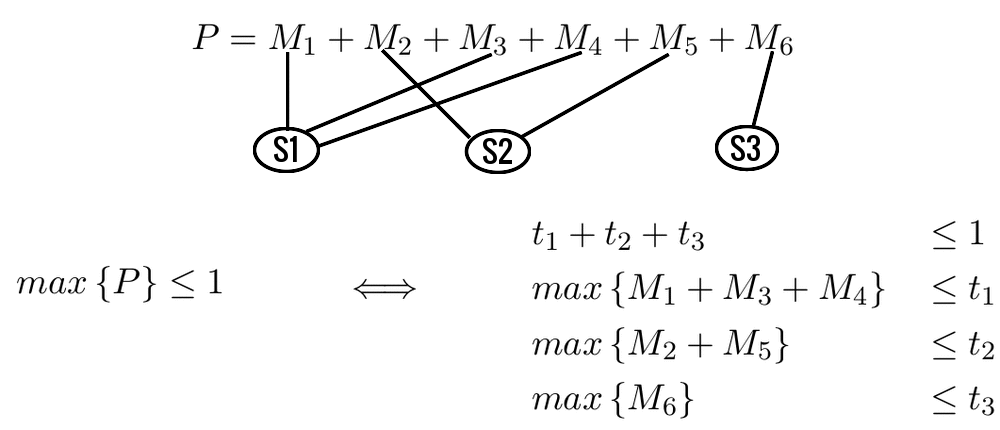
\includegraphics[scale=0.25]{partitioning.png}
	\end{center}
	\caption{Example of partitioning a large posynomial into smaller posynomials.}
	\label{partitioning}
\end{figure}

The posynomial constraints are categorized into three sets: monomials, two-term posynomials, and large posynomials. Monomials are tractable, and two-term posynomials can be well approximated using piecewise-linear functions \cite{hsiung_kim_boyd_2007}. Finding tractable approximations for large posynomials will be summarized next.
\subsection{Linearized Perturbations Formulation}
If the exponents are known and certain, then large posynomial constraints can be approximated as signomial constraints. \\
The exponential perturbations in each posynomial are linearized using a modified least squares method, and then the posynomial is robustified using techniques from robust linear programming. The resulting set of constraints is \gls{sp} compatible, therefore, a robust geometric program can be approximated as a signomial program.

\subsection{Best Pairs Formulation}

%TODO
WORK IN PROGRESS.

%\subsection{Two Term Formulation}
